\section{Introduction}

At some point in their academic journey, every student faces the challenge of selecting the elective courses required for graduation. Choosing the right "free choice" exam is difficult for several key reasons:

\begin{itemize}
	
	\item \textbf{Informative gap}: a major hurdle is the lack of up-to-date and relevant information regarding course material, examination formats, and the actual workload involved. Without these details, making an informed decision is nearly impossible.
	
	\item \textbf{Community experience}: the opinions of former students are essential for determining if a course aligns with one's academic goals and timeline. Unfortunately, it is often difficult to locate peers on campus or in online chats who are available to provide honest, detailed answers about specific subjects.
	
	\item \textbf{Professor competence}: the quality of a course is largely determined by a professor's teaching ability and their availability to students. It is nearly impossible to gauge a professor’s effectiveness without attending their lectures; however, this information is needed at the start of the semester, not at the end, when study plans are already locked and time has run out.
	
\end{itemize}

\noindent The solutions to all these problems is \textbf{EduMeter}, a platform made for students by students. 

\subsection{Statement}

\textbf{EduMeter} is a dedicated web platform for bachelor’s and master’s students at the University of Florence. It serves as a central hub for viewing and publishing reviews of university courses, fostering a transparent academic community. \\

The system categorizes users into three distinct roles, each with specific permissions and capabilities:

\begin{itemize}

    \item \textbf{Guest User}: unauthenticated users can browse the entire collection of course reviews. To ensure ease of navigation, guests can apply various filters to search through review content and metadata.
	
	\item \textbf{Student User}: once authenticated via a personal institutional email, students can browse the corpus and post new reviews. To encourage honest feedback, all student identities remain strictly anonymous within the platform. The community of students can choose to up-vote the best reviews and also report unfair behaviors to the Admin. 
	
    \item \textbf{Admin}: this administrative role is responsible for overseeing the platform's integrity. Admins verify the information submitted by students and hold full CRUD (Create, Read, Update, Delete) permissions to manage the system’s data records. Moreover, the Admin has to duty to ban the reported users from the platform. Every operation is performed on a separate control panel which the Admn can log into with his personal verified email.

\end{itemize} 

\vspace{.7em}
		
\begin{figure}[H]
	
	\centering
	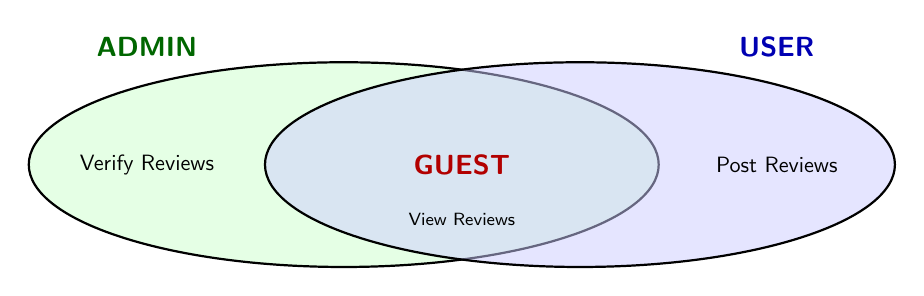
\begin{tikzpicture}[thick, font=\sffamily]
		
		% 1. ADMIN Ellipse (Left - Green)
		\draw[fill=green!20, fill opacity=0.5] (0,0) ellipse (4cm and 1.3cm);
		\node[text=green!40!black] at (-2.5, 1.5) {\textbf{ADMIN}};
		
		% 2. USER Ellipse (Right - Blue)
		\draw[fill=blue!20, fill opacity=0.5] (3,0) ellipse (4cm and 1.3cm);
		\node[text=blue!70!black] at (5.5, 1.5) {\textbf{USER}};
		
		% 3. GUEST Label (Placed in the intersection)
		% The intersection center is roughly at (1.5, 0)
		\node[text=red!70!black] at (1.5, 0) {\textbf{GUEST}};
		
		% --- Example Permissions ---
		\node[scale=0.8] at (-2.5, 0) {Verify Reviews}; % Admin Only side
		\node[scale=0.8] at (5.5, 0) {Post Reviews};   % User Only side
		\node[scale=0.8] at (1.5, -0.7) {\footnotesize View Reviews}; % Guest (Intersection)
		
	\end{tikzpicture}
	\caption{Permission overlap Venn Diagram with some examples of permitted actions per user category.}
	
\end{figure}

To ensure consistency and data integrity, each review follows a standardized structure. Students must complete the following numerical and string fields to submit their feedback:

\begin{itemize}
	\item \textbf{School}: the specific school in which the student is currently a candidate for a degree.
	\item \textbf{Degree}: up-to-date enrolled degree of the reviewer.
	\item \textbf{Teacher}: name of the teacher who held the course.
	\item \textbf{Course}: name of the subject being reviewed.
	\item \textbf{Difficulty}: numerical value representing the student's perceived course difficulty.
	\item \textbf{Enjoyment}: numerical value indicating the reviewer's overall course enjoyment.
	\item \textbf{Comment}: text field for providing detailed qualitative feedback.
\end{itemize} 

\subsection{System architecture and tools}\label{system-architecture-section}

EduMeter is a web application divided into two distinct parts that rely on several industrial-grade libraries to ensure scalability, security, and modularity:

% ? An SMTP server is required for authentication, which consists of an OTP (One Time Pin) being sent to the address that has an allowed domain (e.g. @edu.unifit.it). Once logged in, the backend provides a JWT (JSON Web Token), which is meant to identify the user in subsequent comunications.

% ?It is important to note that the User Identifier (userID) is obtained through hashing the email chained to a secret key. This garantuees the anoniminity of students, but still allows to ban certain userIDs that have been flagged for unfair conduct.

\paragraph{\textbf{Backend.}}
This part is responsible for managing the core application logic, interfacing with a PostgreSQL database and auxiliary servers for external services, such as SMTP. Developed in Java, it exposes a RESTful HTTP API to facilitate client-side communication. The codebase is organized into three primary packages to ensure modularity and separation of concerns:

\begin{itemize}
	\item \textbf{Business Logic}: Contains the application’s functional requirements, including \textbf{REST} endpoints, and \textbf{authentication management}. While the physical SMTP server is not yet integrated, the system includes a fully defined \textbf{SMTP Interface}. This abstraction decouples the business logic from the specific mail provider, allowing a concrete SMTP implementation to be "swapped in" with zero modifications to the core application code. This ensures the system remains extensible and easily testable using mock mail services. To ensure data security, \textbf{HMAC} is utilized as a robust mechanism for verifying and securing sensitive user and administrator information.
	\item \textbf{Domain Model}: Defines the system's core entities. Following the principle of encapsulation, each entity is responsible for maintaining its own internal state and data consistency.
	\item \textbf{DAO (Data Access Object)}: Abstracts the persistence layer from the business logic. This package manages entity lifecycle and database interactions. Additionally, an \textbf{in-memory storage system} is implemented to provide a lightweight testing environment that remains independent of the production database.
\end{itemize}

\begin{figure}[H]
	\centering
	\begin{tikzpicture}[thick, font=\sffamily]

	\begin{umlpackage}[x=2.5, y=-1]{Business Logic}
		\begin{umlpackage} {auth} \end{umlpackage}
		\begin{umlpackage}[x=3] {controllers} \end{umlpackage}
		\begin{umlpackage}[x=2,y=-3] {exception} \end{umlpackage}
	\end{umlpackage}
	\begin{umlpackage}[x=12, y=-4]{Domain Model}\end{umlpackage}
	\begin{umlpackage}[x=9.5]{ORM}
		\begin{umlpackage} {Postgre} \end{umlpackage}
		\begin{umlpackage}[x=3] {InMem} \end{umlpackage}
		\begin{umlpackage}[x=6.5] {DAO interface} \end{umlpackage}
	\end{umlpackage}

	\umlimport[geometry=|-, anchor1=east, anchor2=west]{Business Logic}{Domain Model}
	\umlimport[geometry=-|, anchor2=-160]{Business Logic}{ORM}
	\umlimport[geometry=|-, anchor1 = -157, anchor2=170]{ORM}{Domain Model}

	% DB node
	\node[cylinder, 
		shape border rotate=90, 
		draw, 
		minimum height=2.5cm, 
		minimum width=2cm, 
		aspect=0.25, 
		fill=gray!10, 
		align=center] (db) at (16, -4) {PostgreSQL\\Database};

	\draw[<->, >=latex, line width=1pt] (db.north) -- (db.north |- ORM.south)
	node[midway, right] {JDBC};

	\end{tikzpicture}
	\caption{UML diagram of the complete code-base. Comprehensive of each component and relationship between each.}
	\label{UML-overall-diagram}
\end{figure}

\paragraph{\textbf{Frontend.}} This component represents the user-facing interface of the platform, specifically tailored for the student body. While the full implementation of the frontend was considered out of scope for the current phase of the project, a comprehensive set of mock-ups is provided in section \ref{mock-ups} to illustrate the intended final product. The interface design prioritizes a seamless UX; every element has been created to guide the user intuitively through the processes of browsing and publishing reviews. 

\paragraph{\textbf{Libraries.}} 

\begin{itemize}
	\item JAX-RS for REST API.
	\item JDBC for database connectivity.
	\item Glassfish for Jakarta EE open source implementation.
	\item Mockito for testing.
\end{itemize}

\noindent Developed using:

\begin{itemize}
	\item Intellij Idea as the main IDE.
	\item Insomnia as a REST testing client.
	\item AI models to automate boring repetitive coding.
\end{itemize}
